% Beispiel Plot: Einschwingvorgang, Unterteilung in flüchtigen und eingeschwungenen Zustand 
% u(t) = u_e(t) + u_f(t) = U0 - exp(-t/tau) 
% mit y= u/U0 und x = t/tau
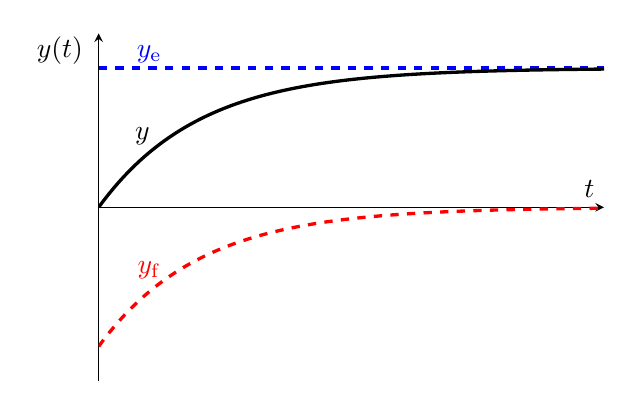
\begin{tikzpicture}
    \begin{axis}[
        xmin=0, xmax=5,
        ymin=-1.25, ymax=1.25,
        xlabel={$t$},
        ylabel={$y(t)$},
		axis x line=center,
		axis y line=center,
		ylabel style={anchor=east, at={(ticklabel cs:0.95)}},% yaxis label left of axis, below arrow tip
        ytick={0},
        yticklabels={0},
        xtick=\empty,
        width=8cm,
        height=6cm,
    ]
        \addplot[very thick, domain=0:5, samples=100, color=blue,dashed]{1};% eingeschwungen
        \addplot[very thick, domain=0:5, samples=100, color=red, dashed]{-exp(-x)};% flüchtig
        \addplot[very thick, domain=0:5, samples=100, color=black]      {1-exp(-x)}; % gesamt
        \node at (0.5,1.1) [blue] {$y_{\mathrm{e}}$};
        \node at (0.5,-0.45) [red]  {$y_{\mathrm{f}}$};
        \node at (0.5,+0.50) [black]{$y_{\phantom{f}}$};
    \end{axis}
\end{tikzpicture}